\section{Fundamentals of Stereo Vision}
\label{sec.stereo}

There are two primary factors to generate a 3D stereo vision, convergence and binocular parallax~\cite{okoshi2012}. The convergence is the angle formed by the eyes and the observed object. The higher the angle value is, the nearer the object is perceived, and vice versa. Therefore, when the convergence is fixed, any object between the eyes and the convergence point will be closer, while the object beyond the convergence point will be farther away. If the convergence is higher then $6^{\circ}$, the eyes feel uneasy~\cite{Fernando2004}. On the contrary, when the value is too small, the stereo sensation will be lost.

Binocular parallax is the difference of images seen by each eye when viewing a scene, creating a sense of depth~\cite{li2012}. The	parallax images are the images passing through to left and right eyes. All 3D stereo media contain a pair of parallax images that are projected on the display, as in Figure~\ref{fig.stereo_parallaxes}. If the images in the pair superimpose, then the binocular focus is on the plane of the images and there is zero parallax.

The positive parallax happens when the target object offsets to the left in the left image, and offsets to the right in the right image, then the binocular focus is lead to fall behind the display, shown in Figure~\ref{fig.stereo_parallaxes}. On the opposite case, the binocular focus is in front of the display, the target offsets are reversed, causing a negative parallax illustrated in Figure~\ref{fig.stereo_parallaxes}.

\begin{figure}
\centering
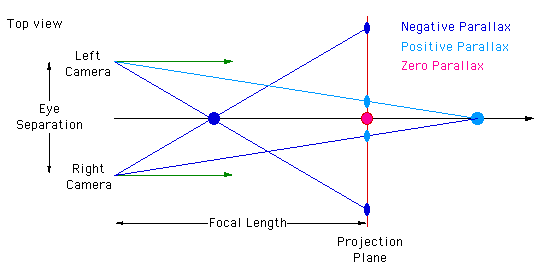
\includegraphics[width=0.8\linewidth,keepaspectratio=true]{figs/stereo_parallaxes.png}

%\begin{tabular}{ccc}
%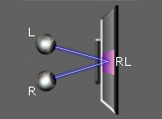
\includegraphics[width=0.3\linewidth,keepaspectratio=true]{figs/zero_parallax.png}
%&
%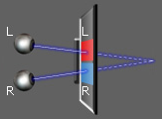
\includegraphics[width=0.3\linewidth,keepaspectratio=true]{figs/positive_parallax.png}
%&
%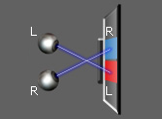
\includegraphics[width=0.3\linewidth,keepaspectratio=true]{figs/negative_parallax.png}
%\\
%(a)&(b)&(c)\\
%\end{tabular}
\caption{Zero, positive and negative stereo parallaxes. }
\label{fig.stereo_parallaxes}
\end{figure}

\subsection{Stereo Displays}
\label{sec.stereo_displays}

The technology for the projection of stereo imagery needs to display (at least) two separate images for left and right eye, respectively, with adequate separation in order to avoid crosstalk or “ghosting”~\cite{Fernando2004}. In general, all existing stereo technology displays the simultaneous projection of two images, so that only one stereo view point can be displayed. 

%In auto-stereographic displays, the emitted viewing rays are blocked or not by a parallax barrier in front of the display, or diverted by a lenticular screen~\cite{Konrad2007}. Although that, only two view points are necessary to create the stereo image pair. A lot of auto-stereographic technologies have been proposed but only few are ready for the end user~\cite{Harris2010}. 

In modern stereo displays, each stereo view point is combined in several ways on the screen; with intertwined lines or squares, combined in even-odd line positions or chessboard pattern respectively; with split screen, divided horizontally or vertically, where each view point is assigned to the respective split side; and with temporal modulation, that requires synchronization with the view polarization apparatus, in the common case stereo glasses with active shutters. Glasses without synchronization relies on passive polarization, that works for all but latter stereo view combination and doubles the resolution per inch halving the amount of pixels.

Active stereo with shutters is based on the principle that the left and right eye images are projected sequentially by a single projector, and that the viewers wear shutter glasses to selectively view the left and right eye images. In order to achieve a good, flicker-free image, the refresh rate needs to be at least 96 Hz (which yields 48 Hz per eye)~\cite{Fernando2004}. The good aspect is, only one display is required for the projection of both left and right images and the effect is independent on the screen type that is used. The drawback are the glasses, which are heavy, cumbersome and needs constant line-of-sight connection with the infrared emitter. Some users also report headaches after extended use.

Passive stereo based on light polarization is a very straightforward technology, using the fact that polarized lenses block the perpendicular light whereas parallel light is transmitted. In its most simple implementation, polarized lenses are mounted in any type of projector. 

%Recent development~\cite{Fernando2004}, using spectral filters to separate between the left and right eye images. This combines the benefits of active and passive: a regular screen can be used, the glasses are lightweight and passive, and the separation is excellent in a restricted angle of viewing.